\section{Introduction}

\begin{figure*}[t]
    \centering
    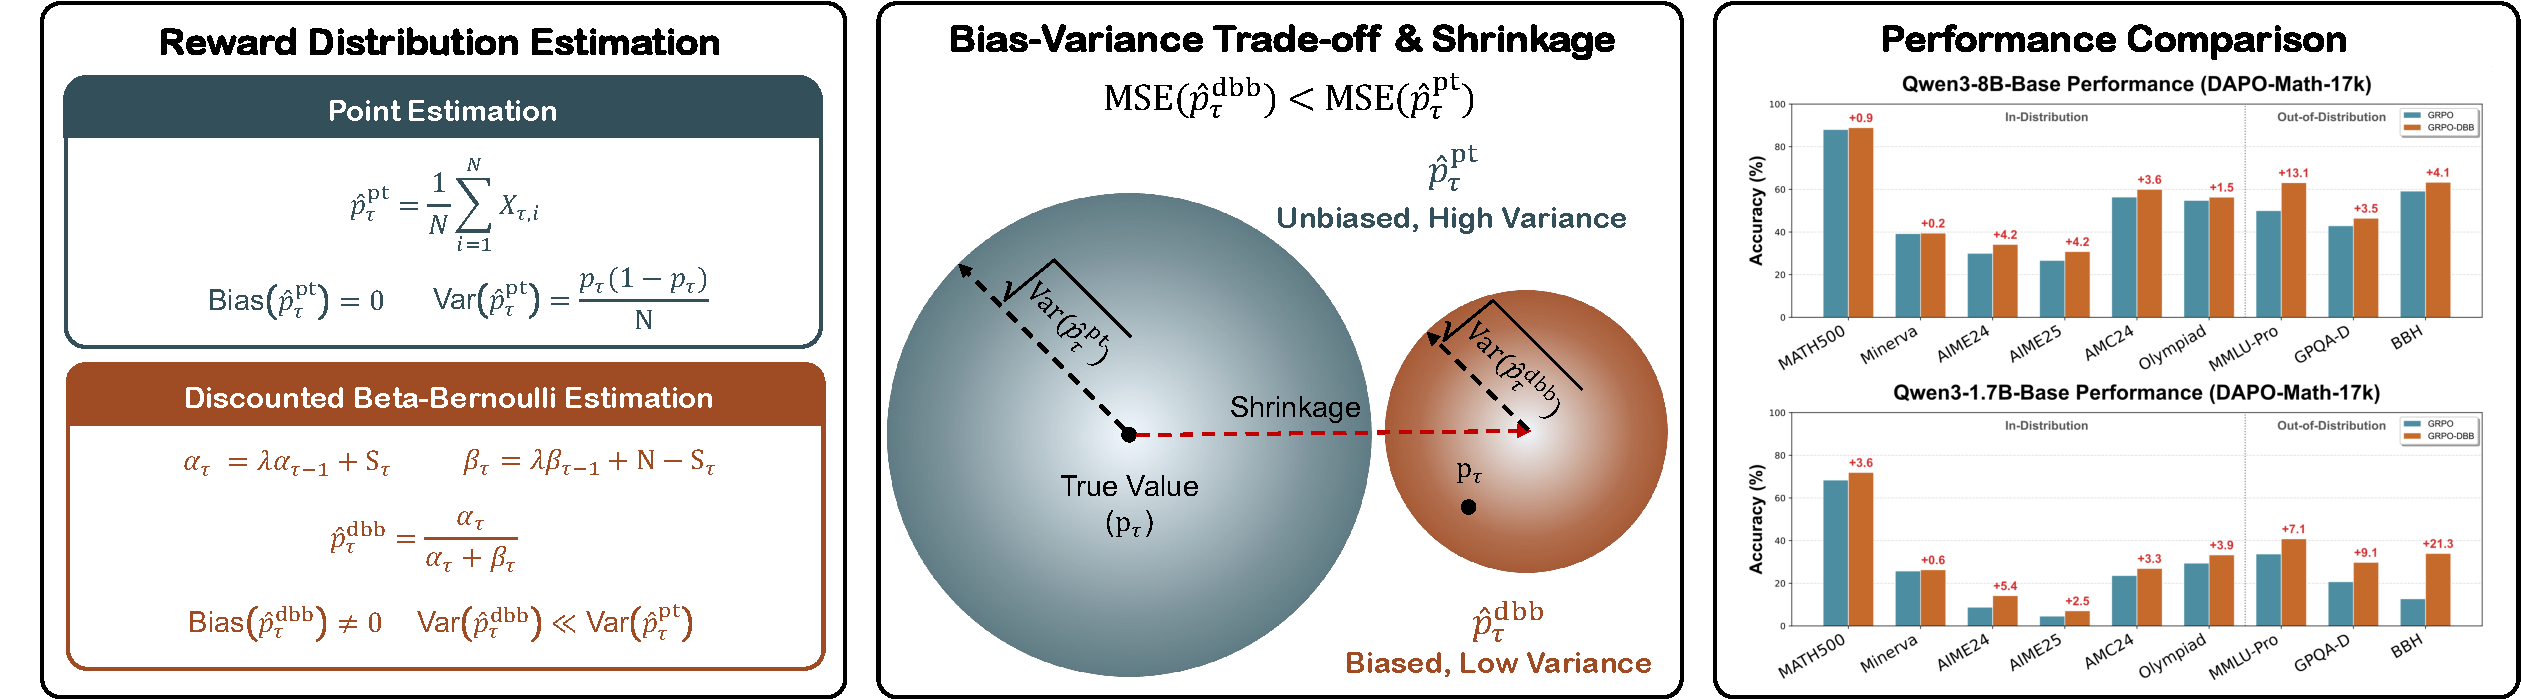
\includegraphics[width=\textwidth]{figures/intro_figure.pdf}
    \caption{Comparison between point estimation and DBB estimation. By trading a small bias for substantial variance reduction via shrinkage, DBB estimation achieves lower mean squared error. Compared to naive GRPO using point estimation, GRPO with DBB estimation consistently demonstrates superior performance across all benchmarks and both model scales.}
    \label{fig:intro_figure}
\end{figure*}

RLVR \cite{lambert2025tulu3pushingfrontiers} has recently emerged as a key post-training paradigm for enhancing the complex reasoning capabilities of large language models \cite{plaat} and improving their performance on downstream tasks \cite{guo2025deepseek, yang2025qwen3technicalreport, yu2025rlprextrapolatingrlvrgeneral}.
Since most RLVR algorithms, including Group Relative Policy Optimization (GRPO; \citeauthor{shao2024deepseekmath}, \citeyear{shao2024deepseekmath}), rely on group-based advantage estimation \cite{yu2025dapoopensourcellmreinforcement, liu2025understandingr1zeroliketrainingcritical, zheng2025groupsequencepolicyoptimization, zhao2025geometricmeanpolicyoptimization}, they require generating multiple responses per prompt, which can account for a large fraction of the overall training time, often approaching 50\% \cite{le2025promptleftbehindexploiting}.
Despite this substantial computational cost, many existing group-based RLVR algorithms fail to utilize information from the generated responses efficiently.


This sample inefficiency can be attributed to two fundamental characteristics of RLVR.
The first characteristic is that the variance of rewards can collapse to zero when all generated responses receive identical rewards under group-relative estimation. 
This \emph{variance collapse} issue not only wastes the computational cost of response generation but also eliminates meaningful training signals within the batch \cite{zhang2025improving}.
To address this issue, approaches such as dynamic sampling \cite{yu2025dapoopensourcellmreinforcement} and GRPO with Efficient Selective Rollout (GRESO; \citeauthor{zheng2025actpaysefficientreinforcement}, \citeyear{zheng2025actpaysefficientreinforcement}) have been proposed. However, dynamic sampling requires several times more rollout cost, and GRESO cannot fully resolve the problem since it probabilistically filters prompts that are likely to result in variance collapse.

The second characteristic is that, due to the on-policy nature of RLVR algorithms, information from all generated responses is discarded after a single gradient update. 
Recent replay-based methods \cite{li2025reporeplayenhancedpolicyoptimization, zhan2025exgrpolearningreasonexperience} attempt to reuse rollouts generated from the training history.
However, unbiased reuse of off-policy data requires importance sampling, which in turn necessitates storing all token-level probabilities under historical policies and performing additional forward passes on the current policy. 
As a result, replay-based approaches introduce substantial GPU memory overhead and additional computational cost, limiting their practical scalability.

These two sources of sample inefficiency primarily arise because most group-based RLVR algorithms rely on point estimators that consider only the rewards from the current rollout group when estimating the underlying reward distribution for advantage estimation. 
While such estimators can be reliable when the number of sampled responses per group is sufficiently large \cite{casella2024}, practical RLVR settings often operate in low-sample regimes due to computational constraints.
In these settings, point estimators remain unbiased but suffer from high variance, which can lead to variance collapse and unstable training dynamics.
% More broadly, existing group-based RLVR approaches have largely emphasized the construction of advantage estimators, while the underlying problem of reward estimation has received comparatively less explicit consideration.


To address this limitation, we adopt a statistical perspective that models rewards as stochastic outcomes drawn from a distribution induced by the policy. 
Instead of relying on point estimation, we employ a Bayesian framework \cite{gelman1995bayesian} to model uncertainty explicitly and incorporate temporal reward dynamics.
Within this framework, we propose the \textbf{D}iscounted \textbf{B}eta--\textbf{B}ernoulli (\textbf{DBB}) reward estimation, which tracks the evolving reward distribution by discounting historical observations. 
While DBB introduces a small bias, it significantly reduces variance and avoids variance collapse, thereby providing more stable and informative training signals (\cref{fig:intro_figure}). 
Empirically, DBB yields a lower mean-squared error with respect to the true reward distribution than point estimation in low-sample scenarios.
% We further demonstrate empirically that the DBB process achieves a lower mean squared error of its estimator than point estimation when the number of rollouts $N$ is small (Section~\ref{sec:mse_analysis}).

We evaluate GRPO with the DBB reward estimator (GRPO-DBB) on two model scales, Qwen3-1.7B-Base and Qwen3-8B-Base \cite{yang2025qwen3technicalreport}, across six in-distribution mathematical reasoning benchmarks, including MATH500, Minerva, AIME24/25, AMC24, and OlympiadBench.
GRPO-DBB consistently outperforms naive GRPO and other baselines across all benchmarks and model sizes.
Specifically, compared to GRPO, GRPO-DBB achieves average Acc@8 improvements of 3.22 and 2.42 points on Qwen3-1.7B-Base and Qwen3-8B-Base, respectively.
Furthermore, on three out-of-distribution reasoning benchmarks such as MMLU-Pro, GPQA-Diamond, and Big-Bench Hard, GRPO-DBB yields average Acc@8 gains of 12.49 and 6.92 points over GRPO on 1.7B and 8B models, respectively.
